% Source: AESP_466_ClassWork/Supplements/Notes/latex/1.3/1.3.tex

\documentclass[border=4pt]{standalone}
\usepackage{amsmath,amssymb}
\usepackage{tikz}

\begin{document}
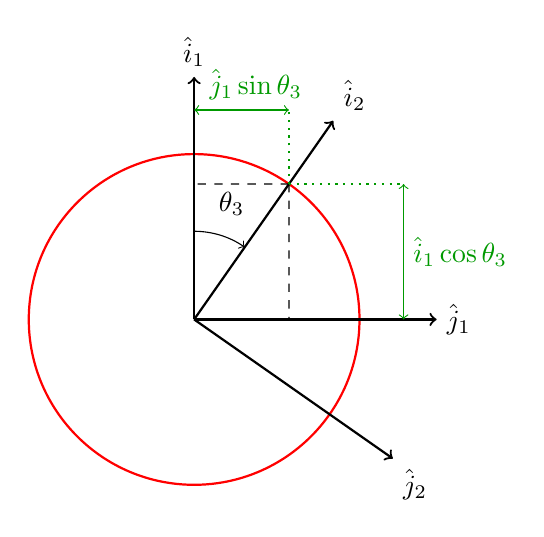
\begin{tikzpicture}[scale=1.4]
    % Draw circle (red like original)
    \draw[thick, red] (0,0) circle (1.5);

    % Frame 1 axes (black)
    \draw[->, thick] (0,0) -- (0,2.2) node[above] {$\hat{i}_1$};
    \draw[->, thick] (0,0) -- (2.2,0) node[right] {$\hat{j}_1$};

    % Frame 2 axes (rotated by theta_3 from Frame 1)
    \draw[->, thick] (0,0) -- (55:2.2) node[above right] {$\hat{i}_2$};
    \draw[->, thick] (0,0) -- (-35:2.2) node[below right] {$\hat{j}_2$};

    % Angle arc between i1 and i2
    \draw[->] (90:0.8) arc (90:55:0.8);
    \node at (72:1.1) {$\theta_3$};

    % Point where i2 intersects circle
    \coordinate (P) at (55:1.5);

    % Projection lines from P to axes (dashed black)
    \draw[dashed] (P) -- (0,{1.5*sin(55)});
    \draw[dashed] (P) -- ({1.5*cos(55)},0);

    % Green dotted vertical line extending UP from P to y=1.9
    \draw[green!60!black, dotted, thick] ({1.5*cos(55)},{1.5*sin(55)}) -- ({1.5*cos(55)},1.9);

    % Green dotted horizontal line extending RIGHT from P to x=1.9
    \draw[green!60!black, dotted, thick] ({1.5*cos(55)},{1.5*sin(55)}) -- (1.9,{1.5*sin(55)});

    % Horizontal dimension arrow: at top of vertical dotted line (y=1.9)
    \draw[<->, green!60!black] (0,1.9) -- ({1.5*cos(55)},1.9);
    \node[green!60!black, above] at ({0.65*1.5*cos(55)},1.9) {$\hat{j}_1\sin\theta_3$};

    % Vertical dimension arrow: at right end of horizontal dotted line (x=1.9)
    \draw[<->, green!60!black] (1.9,0) -- (1.9,{1.5*sin(55)});
    \node[green!60!black, right] at (1.9,{0.5*1.5*sin(55)}) {$\hat{i}_1\cos\theta_3$};
\end{tikzpicture}
\end{document}
